% \documentclass[aip,jcp,preprint,unsortedaddress,a4paper,onecolum]{revtex4-1}
\documentclass[aip,jcp,a4paper,reprint,onecolumn]{revtex4-1}
% \documentclass[aps,pre,twocolumn]{revtex4-1}
% \documentclass[aps,jcp,groupedaddress,twocolumn,unsortedaddress]{revtex4}

\usepackage[fleqn]{amsmath}
\usepackage{amssymb}
\usepackage[dvips]{graphicx}
\usepackage{color}
\usepackage{tabularx}
\usepackage{algorithm}
\usepackage{algorithmic}

\makeatletter
\makeatother

\newcommand{\recheck}[1]{{\color{red} #1}}
\newcommand{\redc}[1]{{\color{red} #1}}
\newcommand{\bluec}[1]{{\color{blue} #1}}
\newcommand{\vect}[1]{\textbf{\textit{#1}}}
\newcommand{\dd}[1]{\textsf{#1}}

\newcommand{\AT}{{\textrm{{AT}}}}
\newcommand{\EX}{{\textrm{EX}}}
\newcommand{\CG}{{\textrm{CG}}}
\newcommand{\HY}{{\Delta}}



\begin{document}

\title{The theoretical considerations on the AdResS}
\author{Han Wang}
% \affiliation{Institute for Mathematics, Freie Universit\"at Berlin, Berlin, Germany}
\author{Carsten Hartmann}
\author{Christof Sch\"utte}
% \affiliation{Institute for Mathematics, Freie Universit\"at Berlin, Berlin, Germany}
\author{Luigi Delle Site}
% \affiliation{Institute for Mathematics, Freie Universit\"at Berlin, Berlin, Germany}

\begin{abstract}
\end{abstract}

\maketitle

\section{Theoretical considerations}
\subsection{The outline of the basic idea}
Here we denote the degrees of freedoms and number of particles in the
atomistic region (AT), hybrid region ($\HY$) and the coarse-grained
region (CG) by $(\vect x_1, N_1)$, $(\vect x_2, N_2)$ and $(\vect x_3,
N_3)$, respectively. Therefore, the target is to prove the atomistic
region is subject to the grand-canonical ensemble: 
\begin{align}
  p(\vect x_1, N_1) = \frac{1}{\mathcal Q_1}
  e^{\beta\mu_{\AT} N_1 - \beta \mathcal H_{N_1}^{\AT}(\vect x_1)} 
\end{align}
where the partition function $\mathcal Q_1$ is defined by
\begin{align}
  \mathcal Q_1 =
  \sum_{N_1}\int
  \dd d\vect x\,
  e^{\beta\mu_{\AT} N_1 - \beta \mathcal H_{N_1}^{\AT}(\vect x_1)}
\end{align}
Let us consider:
\begin{align}
  p(\vect x_1, N_1) = p(\vect x_1 | N_1)\,p(N_1)
\end{align}
rigorously speaking, for a truly grand-canonical ensemble, $p(\vect x_1 | N_1)$ and $p(N_1)$
should be
\begin{align}\label{eqn:p-1}
  p(\vect x_1 | N_1) &= \frac{1}{Q_{N_1}} e^{-\beta \mathcal H_{N_1}^{AT}(\vect x_1)} \\\label{eqn:p-2}
  p(N_1) &= \frac{1}{\mathcal Q_1}e^{\beta\mu_{AT} N_1}Q_{N_1}
\end{align}
where $Q_{N_1}$ is the partition function for a canonical ensemble
with $N_1$ atomistic molecules:
\begin{align}
  Q_{N_1}  =
  \int\dd d\vect x\,
  e^{ - \beta \mathcal H_{N_1}^{\AT}(\vect x_1)}
\end{align}
It must be kept in mind that we always compare the distributions of the AdResS simulation
with a those of a full atomistic reference system, which is ideally divided
in subregions corresponding to the AT, $\HY$ and CG regions of the AdResS
simulation. The first step in our procedure is to fix the number of molecules in the atomistic
region and consider the conditional probabilty $p(\vect x_1 |
N_1)$. If the AdResS set up, leads to the Grand Canonical ensemble, this
probabilty should be the same as the corresponding one of a full
atomistic reference system, namely Eqn.~\eqref{eqn:p-1} (natual Grand Canonical).  Then, if the
probablity of finding $N_1$ molecules in the atomistic region is also
the same as the full atomistic reference system, namely
Eqn.~\eqref{eqn:p-2}, we can savely state that the atomistic region of AdResS
samples configurations in a Grand Canonical fashion.


\subsection{Probability $p(\vect x_1 | N_1)$}
To prove the statement above, the probability $p(\vect x_1 | N_1)$ is divided into two parts:
\begin{align}
  p(\vect x_1 | N_1) = \sum_{N_2}\int
  p(\vect x_1 | N_1; \vect x_2, N_2) \,
  p(\vect x_2, N_2 | N_1)
  \,\dd \vect x_2
\end{align}
$p(\vect x_1 | N_1; \vect x_2, N_2)$ is the probability obtained by fixing the
coordinates and number of particles in the region $\HY$ and considering
the distribution of the DOFs in the AT region. As we have shown before,
if we modify the weighting function by
\begin{align}\label{eqn:new-w}
  w(\vect r) =
  \left\{
    \begin{array}{lcl}
      1 &\quad& \chi < d_{\textrm{ex}}\\
      1  && d_{\textrm{ex}} < \chi < d_{\textrm{ex}} + r_c\\
      \cos^2\big[\frac{\pi}{2(d_{\textrm{hy}} - r_c)} (\chi - d_{\textrm{ex}} - r_c)\big] && d_{\textrm{ex}} + r_c < \chi < d_{\textrm{ex}} + d_{\textrm{hy}} \\
      0 && d_{\textrm{ex}} + d_{\textrm{hy}}  < \chi.
    \end{array}
  \right.
\end{align}
We can prove:
\begin{align}
  p(\vect x_1 | N_1; \vect x_2, N_2)
  \propto &\,
  e^{-\beta\mathcal H_{N_1}^{\AT}(\vect x_1; \vect x_2, N_2)}
\end{align}
with an atomistic Hamiltonian:
\begin{align}
  \mathcal H_{N_1}^{{\AT}}(\vect x_1; \vect x_2, N_2) = &\,
  \sum_{j=1}^{N_1}\frac12 m_i\vect v_i^2 + 
  \sum_{i,j=1}^{N_1}\frac12 U^{{\AT}}(\vect r_i - \vect r_j)  +
  \sum_{i=1}^{N_1}\sum_{j=N_1+1}^{N_2} U^{{\AT}}(\vect r_i - \vect r_j)   
\end{align}
which is exactly the same as the full atomistic reference system.  At this point, the key question is that whether the probability in the $\HY$ region, $p(\vect
x_2, N_2 | N_1)$ is the same as that of the full atomistic reference
system. Generally, this seems not be the case, but it is possible to
derive necessary conditions to this aim. The simplest ones invole
the marginal distribution functions, namely
\begin{align}
  \rho_{\HY}(\vect r) &= \rho_{\AT}(\vect r)\\
  g_{\HY}( r) &= g_{\AT}(r)
\end{align}
The first order marginal distribution is the particle (or molecular) density 
$\rho_{\HY}(\vect r)$, while the second order marginal distribution is
the radial distribution function (RDF), $g_{\HY}(r)$. The necessary
conditions are that these two distribution should be the same as those of the fully atomistic reference system.


\subsection{Discussion about the thermodynamic force}
\begin{figure}
  \centering
  \begin{minipage}[t]{0.49\linewidth}
  \includegraphics[width=0.6\textwidth]{fig.grand/partition.eps}    
  \end{minipage}
  % \begin{minipage}[t]{0.49\linewidth}
  % 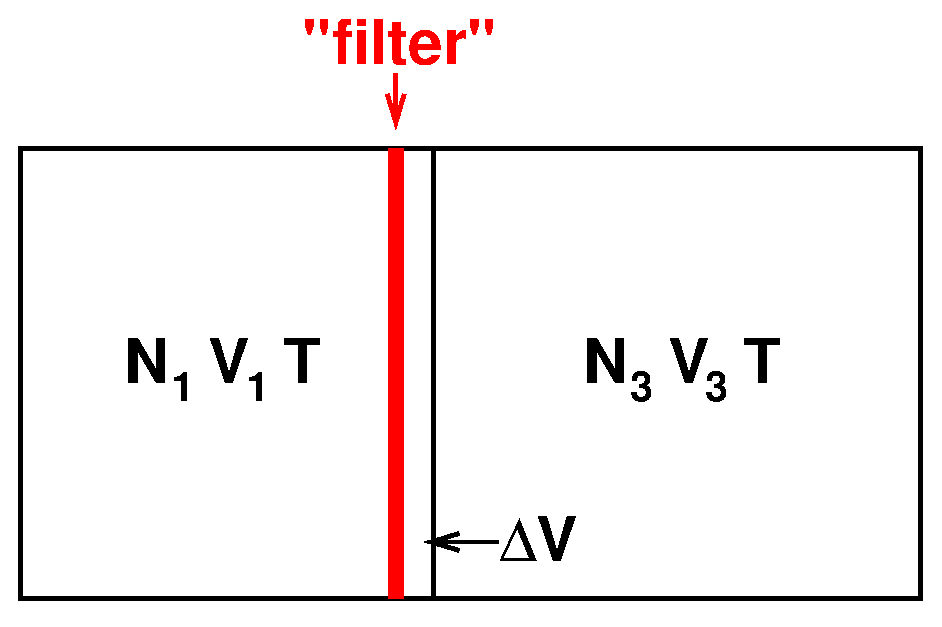
\includegraphics[width=0.6\textwidth]{fig.grand/partition-1.eps}    
  % \end{minipage}
  \caption{Schematic plot of the AdResS system in thermodynamic equilibrium}
  \label{fig:tmp1}
\end{figure}
Here, two assumptions are made:
\begin{enumerate}
\item $N_2\ {\ll}\ N_1 \ll N_3$: the second inequality corresponds to
  the thermodynamic limit of the grand-canonical ensemble. The first
  one actually assumes that the $\HY$ region is infinitely thin so that it
  can be viewed as an infinitesimal membrane that allows free exchange of molecules from
  the AT region to the CG region and vice versa.
\item We now define a supplementary Hamiltonian:
  \begin{equation}
    \mathcal H(\vect x_1, N_1; \vect x_3, N_3) =
    \mathcal H_{N_1}^{\AT}(\vect x_1) + \mathcal H_{N_3}^{\CG}(\vect x_3); 
  \end{equation}
  The condition above is true, in the thermodynamic limit, if the system is
  short-range correlated.
\end{enumerate}
The equilibrium in the AT and CG region is assured by the membrane $HY$ via the thermodynamic force. Conceptually, we assume there is an infinitely thin
``filter'' (see Fig.~\ref{fig:tmp1}) located at the interface between
the AT and CG regions. When a molecule travels from the CG region to
the AT region, the filter does some work $\omega_0$ on the system.
Therefore, we add an empirical term in the Hamiltonian of the system
$N_1\omega_0$, which denotes the work done by the thermodynamic force.  having Fixed the number of molecules in the three regions, and by following the
arguments of the last section, both the AT and the CG regions are
subject to the Boltzmann distribution. Thus, the partition function of the
system reads
\begin{align}\nonumber
  q(N,V,T)
  &= \frac1{N!}\int
  \dd d\vect x
  e^{-\beta
    [\mathcal H(\vect x_1, N_1; \vect x_3, N_3) +
    N_1\omega_0]}\\\nonumber
  &= \frac1{N!}\int
  \dd d\vect x_1\dd d\vect x_3\,
  e^{-\beta
    [\mathcal H_{N_1}^{\AT}(\vect x_1) +
    \mathcal H_{N_3}^{\CG}(\vect x_3) +
    N_1\omega_0]}\\\nonumber
  & = \frac{N_1!N_3!}{N!}
  e^{-\beta N_1\omega_0}
  \frac{1}{N_1!}\int\dd d\vect x_1 e^{-\beta\mathcal H_{N_1}^{\AT}(\vect x_1)}
  \frac{1}{N_3!}\int\dd d\vect x_3 e^{-\beta\mathcal H_{N_3}^{\CG}(\vect x_3)}\\
  & = \frac{N_1!N_3!}{N!}
  e^{-\beta N_1\omega_0}
  Q_{\AT}(N_1, V_1, T)\,
  Q_{\CG}(N_3, V_3, T) 
\end{align}
Considering the permutations of particles, the number of possibilities of
$N_1$ molecules being in the atomistic region and $N_3$ molecules being
in the coarse-grained region is  $\frac{N!}{N_1!N_3!}$.
Therefore, the partition function of the whole system reads
\begin{align}\nonumber
  Q(N,V,T) &= \sum_{N_1}
  \frac{N!}{N_1!N_3!} \frac{N_1!N_3!}{N!}
  e^{-\beta N_1\omega_0}
  Q_{\AT}(N_1, V_1, T)\,
  Q_{\CG}(N_3, V_3, T) \\
  &= \sum_{N_1}
  e^{-\beta N_1\omega_0}
  Q_{\AT}(N_1, V_1, T)\,
  Q_{\CG}(N_3, V_3, T) 
\end{align}
with natural constraints:
\begin{align}
  N &= N_1 + N_3\\
  V &= V_1 + V_3
\end{align}
It can be proved that (see for example
Ref.~\cite{tuckeman2010statistical})
if
\begin{align}
  -\beta N_1\omega_0 +
  \ln Q_{\AT}(\bar N_1, V_1, T) + \ln Q_{\CG}(N - \bar N_1, V_3, T) \gg \ln N 
\end{align}
where
\begin{align}
  \bar N_1 = \underset{N_1}{\textrm{argmax}}\:
  e^{-\beta N_1\omega_0}
  Q_{\AT}(N_1, V_1, T) \,Q_{\CG}(N - N_1, V_3, T)
\end{align}
then
\begin{align}
  \ln Q(N, V, T)
  \approx
  -\beta \bar N_1\omega_0 + 
  \ln Q_{\AT}(\bar N_1, V_1, T) + \ln Q_{\CG}(N - \bar N_1, V_3, T)
\end{align}
or equivalently
\begin{align}\label{eqn:a-energy-1}
  A(N, V, T)
  \approx
  \bar N_1\omega_0 +
  A_{\AT}(\bar N_1, V_1, T) + A_{\CG}(N - \bar N_1, V_3, T)
\end{align}
Where $A$ denotes the Helmhotz free energy.  $\bar N_1$ is the maximum
parameter of $e^{-\beta N_1\omega_0} Q_{\AT}(N_1, V_1, T) \,Q_{\CG}(N - N_1,
V_3, T)$. We will see later that this maximum corresponds to the maximum
value of probability $p(N_1)$; this is also the equilibrium molecular
number in the AT region in the thermodynamic limit.  Since $\bar
N_1$ is the maximum, by differentiation on the right hand side of
Eqn.~\eqref{eqn:a-energy-1}, we have the relation:
\begin{align}
  \omega_0 = \mu_{\CG}(N - \bar N_1, V_3, T)  - \mu_{\AT}(\bar N_1, V_1, T)
\end{align}
That means that the difference in the chemical potential between the AT and CG
regions is taken care by the thermodynamic force.  To ensure an
equilibrium that is the same as the full atomistic reference system,
the work done by the thermodynamic force should be the same as the
chemical potential difference between the atomistic and coarse-grained
resolutions, namely
\begin{align}\label{eqn:w-mu-diff}
  \omega_0 = \mu_{\CG}(\rho_0V_3, V_3, T) - \mu_{AT}(\rho_0 V_1, V_1, T)
\end{align}
$\rho_0$ is the density at which the atomistic and coarse-grained
resolutions should match,
namely $\bar N_1 = \rho_0V_1$ should apply.  This is a necessary
condition for the correct equilibrium of the AT and CG regions.\\

\noindent
Now we translate from the language of Helmhotz free
energy into that of the grand potential.
Under the thermodynamic limit, they are the same.
Assuming the system reaches an
equilibrium of flat density profile of $\rho_0$ all over the AdResS simulation box, 
Eqn.~\eqref{eqn:a-energy-1} becomes:
\begin{align}\label{eqn:g-energy-1}
  G(\mu, V, T) \approx
  \rho_0V_1\omega_0
  + G_{\AT}(\mu_{\AT}, V_1, T) + G_{\CG}(\mu_{\CG}, V - V_1, T)
\end{align}
where
\begin{align}
  G(\mu, V, T) = A(N, V, T) - \mu_{\AT} \bar N_1 - \mu_{\CG}(N - \bar N_1)
\end{align}
Because of the equilibrium situation, dthe erivative of r.h.s. of
Eqn.~\eqref{eqn:g-energy-1} with respect to atomistic volume $V_1$
should vanishes (the same argument as the Helmhotz free energy):
\begin{align}
  \rho_0\omega_0 = -p_{\AT}+p_{\CG} \quad\Longrightarrow\quad
  p_{\AT} + \rho_0\omega_0 = p_{\CG}
\end{align}
which is exactly the definition of the thermodynamic force.


\subsection{The number probability $p(N_1)$}
Now let us consider the marginal distribution $p(N_1)$
\begin{align}\nonumber
  p(N_1)
  % &=
  % \int
  % \dd d\vect x
  % \,e^{-\beta
  %   [\mathcal H(\vect x_1, N_1; \vect x_3, N_3) +
  %   N_1\omega_0]}\\\nonumber
  &=
  \frac{N!}{N_1!N_3!}
  \int
  \dd d\vect x_1\dd d\vect x_3  \:
  \frac{1}{Q(N,V,T) N!}
  e^{-\beta
    [\mathcal H_{N_1}^{\AT}(\vect x_1) +
    \mathcal H_{N_3}^{\CG}(\vect x_3) +
    N_1\omega_0]}\\\nonumber
  &=
  \frac{N!}{N_1!N_3!}
  \frac{N_1!N_3!}{Q(N,V,T) N!}
  e^{-\beta N_1\omega_0}
  \bigg[
  \frac1{N_1!}
  \int
  \dd d\vect x_1
  e^{-\beta \mathcal H_{N_1}^{\AT}(\vect x_1)}
  \bigg]
  \bigg[
  \frac1{N_3!}
  \int
  \dd d\vect x_3
  e^{-\beta \mathcal H_{N_3}^{\CG}(\vect x_3)}
  \bigg]  \\\nonumber
  &=
  \frac
  {
    e^{-\beta N_1\omega_0}
    Q_{\AT}(N_1,V_1,T) Q_{\CG}(N-N_1,V_3,T)
  }
  {
    \sum_{n_1}
    e^{-\beta n_1\omega_0}
    Q_{\AT}(n_1,V_1,T) Q_{\CG}(N-n_1,V_3,T)
  }
\end{align}
The atomistic marginal distribution, which the AdResS simulation should
reporduce is
\begin{align}
  p_{\AT}(N_1)
  &=
  \frac
  {
    Q_{\AT}(N_1,V_1,T) Q_{\AT}(N-N_1,V_3,T)
  }
  {
    \sum_{n_1}
    Q_{\AT}(n_1,V_1,T) Q_{\AT}(N-n_1,V_3,T)
  }  
\end{align}
Multiplying the numerator of $p(N_1)$ by the denominator of
$p_{\AT}(N_1)$, we have the term denoted by $T_1$
\begin{align}\nonumber
  T_1
  &=
  \sum_{n_1}
  e^{-\beta N_1\omega_0}
  Q_{\AT}(n_1,V_1,T)\,
  Q_{\AT}(N_1,V_1,T)\,
  Q_{\AT}(N-n_1,V_3,T)\,
  Q_{\CG}(N-N_1,V_3,T) \\\nonumber
  &=
  \sum_{n_1}
  \exp
  \big\{-\beta
  \big[
  \omega_0N_1 +
  A_{\AT}(n_1,V_1,T) +
  A_{\AT}(N_1,V_1,T) +
  A_{\AT}(N-n_1,V_3,T) +
  A_{\CG}(N-N_1,V_3,T)
  \big]
  \big\}
\end{align}
Since we work under the hypothesis taht the atomistic region is much smaller than the whole system, it
is reasonable to assume $n_1 \ll N$ nad $N_1\ll N$. We have the following
expansions:
\begin{align}
  A_{\AT}(N-n_1,V_3,T)
  &=
  A_{\AT}(N,V_3,T)
  - \mu_{\AT}\,n_1
  + \frac12 \kappa_{\AT}\,n_1^2 + \textrm{h.o.t.} \\
  A_{\CG}(N-N_1,V_3,T)
  &=
  A_{\CG}(N,V_3,T)
  - \mu_{\CG}\,N_1
  + \frac12 \kappa_{\CG}\,N_1^2 + \textrm{h.o.t.}
\end{align}
One should keep in mind the conditions:
\begin{align}\label{eqn:mu-eq}
  \mu_{\CG} &= \mu_{\AT} + \omega_0\\\label{eqn:kappa-eq}
  \kappa_{\CG} &= \kappa_{\AT}
\end{align}
We have $T_1$
\begin{align}\nonumber
  T_1
  = \,&
  \sum_{n_1}
  \exp
  \big\{-\beta
  \big[
  A_{\AT}(n_1,V_1,T) +
  A_{\AT}(N_1,V_1,T) +
  A_{\AT}(N,V_3,T) +
  A_{\CG}(N,V_3,T) \\
  \,&-
  \mu_{\AT}\,(N_1 + n_1) +
  \frac12 \kappa_{\AT}(N_1^2 + n_1^2) +
   \textrm{h.o.t.}
  \big]
  \big\}
\end{align}
Similarly, multiplying the numerator of $p_{\AT}(N_1)$ by the denominator of
$p(N_1)$, we have the term denoted by $T_2$
\begin{align}\nonumber
  T_2
  &=
  \sum_{n_1}
  e^{-\beta n_1\omega_0}
  Q_{\AT}(n_1,V_1,T)\,
  Q_{\AT}(N_1,V_1,T)\,
  Q_{\CG}(N-n_1,V_3,T)\,
  Q_{\AT}(N-N_1,V_3,T) \\\nonumber
  &=
  \sum_{n_1}
  \exp
  \big\{-\beta
  \big[
  \omega_0n_1 +
  A_{\AT}(n_1,V_1,T) +
  A_{\AT}(N_1,V_1,T) +
  A_{\CG}(N-n_1,V_3,T) +
  A_{\AT}(N-N_1,V_3,T)
  \big]
  \big\}
\end{align}
with similar expansions and by noticing the conditions Eqn.~\eqref{eqn:mu-eq}
and \eqref{eqn:kappa-eq}, we have:
\begin{align}\nonumber
  T_2
  = \,&
  \sum_{n_1}
  \exp
  \big\{-\beta
  \big[
  A_{\AT}(n_1,V_1,T) +
  A_{\AT}(N_1,V_1,T) +
  A_{\AT}(N,V_3,T) +
  A_{\CG}(N,V_3,T) \\
  \,&-
  \mu_{\AT}\,(N_1 + n_1) +
  \frac12 \kappa_{\AT}(N_1^2 + n_1^2) +
   \textrm{h.o.t.}
  \big]
  \big\}
\end{align}
Therefore, term $T_1$ and $T_2$ are consistent with  the second leading
order, which means $p(N_1)$ is a good approximation of $p_{\AT}(N_1)$
to the second leading order.



\section*{References}
\bibliography{ref}{}
\bibliographystyle{unsrt}





\end{document}